\documentclass[10pt]{article}
\usepackage{caption}
\usepackage{subcaption}
\usepackage{graphicx}
% \usepackage{multirow}
% \usepackage{wrapfig}
\usepackage{enumerate}
\usepackage{cite}
\usepackage[margin=1.1in]{geometry}

\begin{document}
\title{6.867 Final Project: An overview of convolutional neural networks with the SUN397 scene recognition database}
\author{Michele Pratusevich}
\date{\today}
\maketitle

\section{Introduction}

Collaboration between artificial intelligence, neuroscience, and machine learning resulted in the invention of neural networks for use in classification or prediction tasks. With roots from single-layer perceptrons \cite{rosenblatt_perceptron:_1958} to multi-layer and kernel perceptrons \cite{aizerman_theoretical_1964}, increasing success on non-linear classification tasks (especially related to vision or images) have seen the revival of their popularity among the computer vision community. 

A popular success story is the development of a back-propagation convolutional neural network (CNN) for handwritten digit recognition \cite{lecun_handwritten_1990}. The original data used was approximately 10,000 handwritten digits, classified into one of 10 categories (one category for each digit). This original dataset was later expanded into the MNIST handwritten digit database with over 60,000 examples \cite{lecun_gradient-based_1998}, \cite{li_deng_mnist_2012}. The network used by LeCunn et. al. used the idea of convolution layers - described essentially as features extracted from parts of the image by kernels of varying sizes, generally getting smaller and smaller. The general idea is that these $n \times n$ kernels will `find' specific features in the image. In between, there are layers that perform averaging or weighting of the features that it receives. The final layer is fully-connected to the receptive fields of the previous layer and outputs a probability estimate for the class the image belongs to, meaning it essentially performs a weighted sum of all the inputs it sees for each parameter, with different weight parameters for each predicted class. Improvements to this network have been made incrementally over time, but the error rates on the test set for this initial network was $3.7$ percent. 

The interesting insights from LeCun's simplified architecture \cite{lecun_handwritten_1990} compared to a previous network that had more connections (also designed by LeCun) \cite{lecun_backpropagation_1989} were two-fold: (1) that images could be fed directly into the neural network rather than extracting features, then feeding the features into the network, and (2) knowing a-priori the nature of the classification task can give hints about how to simplify the network to contain fewer parameters to optimize over. In general, these ideas of simplification of neural networks can be applied to larger and more complex neural networks \cite{lecun_optimal_1989}. 

Since LeCun's successful use of CNNs for handwritten digit classification, CNNs became a popular technique for completing computer vision tasks. Krizhevsky et. al. \cite{krizhevsky_imagenet_2012} constructed an 8-layer CNN that achieved 17 percent top-5 error rates on the ImageNet database \cite{russakovsky_imagenet_2014}, taking advantage of optimizations using GPUs and a few other numerical improvements cited in the paper. Since then, very deep CNNs have been used for nearly every computer vision task with a standard dataset, and countless other non-standardized tasks. Since the original AlexNet was published, fine-tunings of the original network, in addition to changes to the architecture, were performed with the hopes of creating a neural network that can be used as a generalized feature extractor for all kinds of image tasks \cite{donahue_decaf:_2014}. Software packages to facilitate this and the use of GPUs for speed-up were created \cite{jia_caffe:_2014}. 

One big problem with using these extremely deep CNNs for feature extraction, fine-tuning, and general image classification tasks is the time needed to train these networks. With GPU speedups and optimized code, this task is made easier, but it still takes approximately 3 days on a GPU to train on the entirety of the ImageNet database (6 million images). Fine-tuning for a specific task using a pre-trained network takes less time, but depending on the desired result takes a few hours. Another big problem with deep CNNs for vision tasks is the need for extremely large quantities of labeled training data. For a large network with 10000s of parameters, having only 50 labeled training images is not enough to optimize over. AlexNet was only able to train from scratch because the training set for ImageNet is incredibly large, with approximately 10,000 images per class and a total of 1000 classes. 

Training neural networks still requires the fine-tuning of hyperparameters dictating the learning rate and the weight decay, but some have offered suggestions for how to improve back-propagation and the choosing of hyperparameters \cite{bottou_large-scale_2010}. However, simultaneously, there have been a number of papers questioning the need for the depth and complexity of the recently-used CNNs \cite{ba_deep_2013}. LeCun provided suggestions for the simplification of neural networks when working with the original handwritten digit classification network \cite{lecun_optimal_1989}. Another interesting area of research has been the idea of using Gaussian processes to optimize parameters in a neural network for a specific task. 

In this project, I will explore the idea of simplified CNNs for the scene recognition vision task, drawing on ideas from recent literature about the effectiveness of using pre-trained networks, simplifying existing networks, and using extracted features to do various tasks. The main concepts I will explore are: 

\begin{enumerate}
	\item The effect of network size on training time 
	\item The effect of kernel size on the learned receptive field and on training time
	\item The process of choosing hyperparameters for learning
\end{enumerate}

The main guiding this exploration is: can you construct a significantly simpler neural network for scene classification that has comparable results to an extremely deep neural network? Decisions in training and parameter tuning will be made to create the smallest network that can be trained in a reasonable amount of time (say 2 hours) to achieve positive results. A general answer to this question is a philosophical question in the field of computer vision, since it touches on the question of whether a highly-specific system that is quick to construct or a highly-general system that is versatile a better outcome. I claim that it depends on the task, but the idea of constructing a simple neural network for complex tasks like scene classification has not been addressed in the literature.

\section{Dataset, Tools, and Related Work}

The task of scene recognition is different from object recognition in that scene recognition relies on clues from the entire image and the general layout rather than specific qualities of objects. The standard dataset for scene recognition is the SUN397 database \cite{xiao_sun_2010}, which has 397 scene categories, with at least 100 images in both categories. The standard train / test splits have 50 images per category in both training and testing. The benchmark classification results on this dataset using hand-crafted features is reported by Xiao, et. al. \cite{xiao_sun_2010}, \cite{xiao_sun_2014}. To build on the SUN397 database is the PLACES database \cite{zhou_learning_2014}, which benchmarks itself against SUN397, and notably uses CNNs for scene classification, rather than hand-crafted features. Because SUN397 has a manageable amount of data to use for training, I will use that database to do tests, benchmarking against the classification rates reported in the SUN papers. The PLACES database and results will provide a second state-of-the-art benchmark for scene classification as well.

To construct the neural networks and take advantage of GPU capabilities, I will use the Caffe software package \cite{jia_caffe:_2014}, optimized for GPU performance and slowly becoming the standard in academic work for building CNNs. There are bindings for C++, Python, and MATLAB, allowing for the use of various interfaces for analysis. The added benefit of using this system is that the PLACES database provides a trained CNN model that can be used for fine-tuning with SUN. Additionally, the Vision Group has a cluster of GPU machines that can effectively run Caffe with some persuasion, so the training times for the networks will be drastically improved over running on a small laptop PC CPU. One of the bottleneck steps in using training data is reading data from disk, so the training and testing sets are converted into LMDB databases optimized for multi-threaded querying. All images are resized to 227 x 227 pixels, in accordance with comparable computer vision experiments. The reason for the small size in images is three-fold: (1) consistent higher-resolution images were only available as standard datasets relatively recently; (2) it has been shown in prior experiments from both neuroscience and computer vision that image-level features do not change significantly when shrunk to this size REFERENCE, and (3) smaller images mean performance increases when reading from disk and computing features over the entire image.

% * CNNs have proven effective in image classification because of the ability to learn high-level features
% * CNN is like a multiclass perceptron?
% 	* start with a single multiclass logistic regression classifier in caffe on SUN
% * http://groups.csail.mit.edu/vision/SUN/
% * neural networks are really networks of logistic regression things
% * multiclass logistic regression on SUN database

% 1. simple logistic regression classifier: network example given here http://caffe.berkeleyvision.org/tutorial/net_layer_blob.html

\section{Method}

The first step in the neural network analysis is to set up Caffe to run on both my personal computer (for small-scale testing and development) and the Vision Cluster (for running experiments). Both proved to be a challenging task because of the need to link highly optimized numerical libraries, resulting in my writing an addendum for how to install Caffe on OSX 10.9 on the Caffe Github wiki.

To set up a single network in Caffe is complicated without knowing the interface, so as a benchmark to start, I constructed a basic logistic regression classifier as a neural network. In the default neural network, activation is computed using the sigmoid function and the loss function is the softmax function.

\begin{figure}[!ht]
\centering
% \begin{subfigure}[b]{0.46\textwidth}
% 	\centering
% 	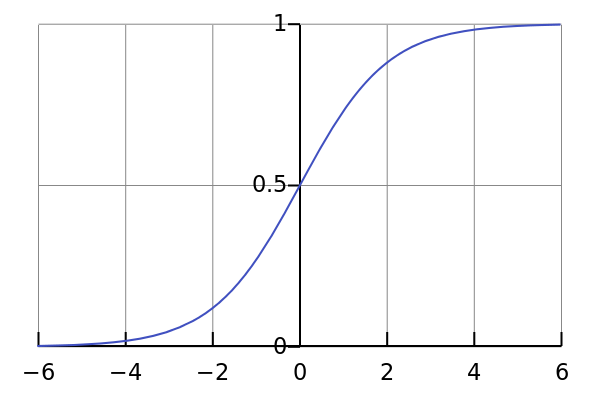
\includegraphics[width=\textwidth]{Logistic-curve.png}
% 	\caption{Sigmoid activation function (taken from Wikipedia)}
% 	\label{fig:sigmoid}
% \end{subfigure}
\begin{subfigure}[b]{0.5\textwidth}
	\centering
	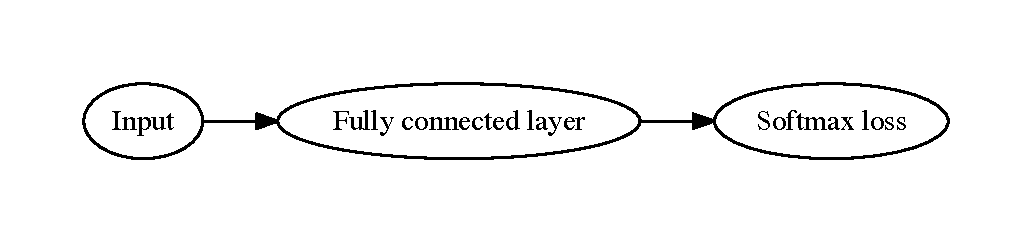
\includegraphics[width=\textwidth]{logreg.pdf}
	\caption{Simplified neural network architecture for logistic regression}
	\label{fig:logregnn}
\end{subfigure}
\begin{subfigure}[b]{0.8\textwidth}
	\centering
	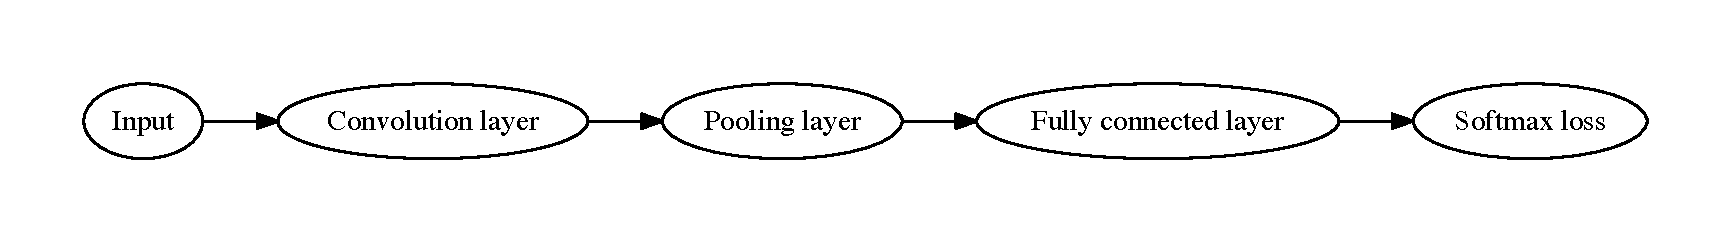
\includegraphics[width=\textwidth]{generalcnn.pdf}
	\caption{General layer structure of a convolutional neural network}
	\label{fig:generalcnn}
\end{subfigure}
\end{figure}

The setup for (linear) logistic regression as a neural network is then represented as shown in Figure \ref{fig:logregnn}. A fully-connected layer is equivalent to calculating weighted sum of dot products between the inputs to the layer, and the softmax function takes these 397 functions and calculates probabilities between them. There are as many layers in the fully-connected network as there are training images, but there are only 397 outputs, meaning there are 397 linear-combinations of functions calculated using weights from the training images. Using stochastic gradient descent to compute the parameters, the optimal learning weight (by grid search and suggestions from Bottou \cite{bottou_large-scale_2010}) was found to be approximately $1 \times 10^{-8}$. On a GPU for 20000 iterations, this takes approximately 15 minutes and results in a top-1 accuracy prediction of 4 percent and a top-5 accuracy prediction of 13 percent. Because simple logistic regression learns relatively few parameters and is only capable of linear combinations of inputs, the idea is that adding any sort of more complicated network will increase this base classification rate. Methods involving more complicated networks were only considered if they yielded results better than this baseline 13 percent top-5 accuracy with logistic regression. 

The standard metric for measuring success against the SUN database is the top-1 classification accuracy rate for correctly predicting with maximum likelihood the correct class. However, because many categories in the SUN397 database are similar (like for example `building exterior' and `apartment building outdoor'), I will also report a top-5 accuracy rate.

After exploring this pipeline using Caffe, for each set of experiments I had to do the following steps: 

\begin{enumerate}
	\item Define the network representation
	\item Define the solver parameters
	\item Define the validation / hyperparameter search procedure
	\item Train the network on the GPU using the training set
	\item Test the network on the GPU using the test set
\end{enumerate}

For all experiments, the same training and test sets were used. 

\section{Experiments}

Because I was limited by computational power and time, for each experiment I chose a few token representations and ran tests on those. The next section will summarize the findings as general conclusions, while here I will report the results and give some observations for specific experiments. A summary of the results of the experiments with best results are given in Table \ref{tbl:results}, along with a comparison of state-of-the-art results. Note that the best result reported in the PLACES-CNN paper \cite{zhou_learning_2014} does not use fine-tuning, but rather features extracted using the CNN fed through an SVM.

\begin{table}[!ht]
\centering
\makebox[\textwidth][c]{
\begin{tabular}[ht]{c|c|c}
Procedure & Top-1 Accuracy & Top-5 Accuracy \\\hline
Logistic regression & 4 \% & 14 \% \\
Best single-layer network &   \% &  \% \\
Best two-layer network &   \% &   \% \\
Simple 3-layer network &    \% &   \% \\
Fine-tuned PLACES CNN & 51.3 \% & 80.1 \% \\
PLACES CNN best SUN397 result & 54.3 \% & not reported \\
\end{tabular}
}
\caption{Summary of top-1 and top-5 accuracy results on the test set}
\label{tbl:results}
\end{table}

\subsection{Single-layer networks of varying kernel size}

For the first set of experiments, single-layer networks with varying kernel size were used. A convolutional layer in a neural network in the context of a computer vision task is similar to training a `receptive field' of an eye. The idea is that some number of $n \times m$ kernels will be computed over the entire image, acting like `filters', then passed to higher layers in the network. In the single-layer network case, the output of the kernel filters are then passed to a fully-connected layer that does a weighted sum of the filters, then passed to a softmax function to predict the probabilities. 

There were a number of numerical issues when approaching the convolution layer problem. For one, having a large number of output filters means that there are an incredibly large vector of numbers passed to the fully-connected layer of the network. Having too many parameters in the vector many means that there is a strong chance that there will not be enough memory to pass these variables around to optimize. Therefore, we use our knowledge of the domain space and of kernels to add an additional layer to the network that both improves performance and decreases training time. Instead of passing all the computed kernels for the entire image to the fully-connected layer, only pass the kernel result that maximally fires for that particular image. This is done in Caffe with `max-pooling'. In general, the structure of networks used is shown in Figure \ref{fig:generalcnn}. 

The kernels that were tested were $8 \times 8$, $12 \times 12$, and $20 \times 20$. AlexNet, PlacesCNN, LeNet, and many other successful CNNs for image tasks use $12 \times 12$ kernels in their first convolutional layer. The kernel that performed the best for a single layer was the $20 \times 20$ kernel. In all cases, there were a total of $96$ kernels computed and a max-pooling layer was then fed into the fully-connected layer. Results for all single-kernel experiments are given in Table \ref{tbl:singlelayer}.

\begin{table}[!ht]
\centering
\makebox[\textwidth][c]{
\begin{tabular}[ht]{c|c|c}
Procedure & Top-1 Accuracy & Top-5 Accuracy \\\hline
96 8$\times$8 kernels, no dropout &  4.8 \% & 14.8 \% \\
96 8$\times$8 kernels, with dropout &  5.7 \% &  15.2 \% \\
96 8$\times$8 kernels, with dropout and RELU & .8 \% & 2 \% \\
96 12$\times$12 kernels, no dropout &  4.4 \% & 13.5 \% \\
96 12$\times$12 kernels, with dropout &  5.5 \% & 15.8 \% \\
96 20$\times$20 kernels, with dropout & 6.7 \% & 18.2 \% \\
30 20$\times$20 kernels, with dropout &  \% &  \% \\
\end{tabular}
}
\caption{Summary of top-1 and top-5 accuracy results on single-layer networks after 20000 iterations}
\label{tbl:singlelayer}
\end{table}

\subsection{Single-layer networks with rectifying linear units}

It has often been cited in successful CNN papers like AlexNet or LeNet \cite{krizhevsky_imagenet_2012}, \cite{lecun_handwritten_1990} that instead of using a sigmoid activation function that a rectified linear function of the form $\max(0, x)$ leads to faster training and improved results, but in 20000 iterations of training on multiple single-layer networks like $8 \times 8$ and $12 \times 12$, the training took approximately double the time than similar networks using sigmoid activation functions and yielded poorer results. So for the rest of the tests, using rectified linear units were not used.

\subsection{Using dropout}

Experiments were also conducted for single-layer networks using dropout layers. It was cited by AlexNet \cite{krizhevsky_imagenet_2012} that dropout layers reduced overfitting. At the output of every convolutional layer, a dropout layer that takes the sample and with probability 0.5 includes it in the resulting output vector. This is equivalent to doing averaging over a number of models to produce a final result. From Table \ref{tbl:singlelayer}, it is clear that dropout layers improve the performance without changing the hyperparameters. Therefore, with all further experiments, dropout layers will be added after every convolutional layer to prevent overfitting. It is especially important to do this when there is not a lot of labeled training data, as with the SUN397 database setup we are using, where there are only 50 labeled images per class.

\subsection{Multi-layer networks}

After the hyperparameters were roughly optimized for single-layer networks, two-layer networks of varying sizes were tried. An additional variable in network design is the decision for how many outputs from each convolutional layer to include. Because each new output adds an additional set of parameters for the network to optimize, the hypothesis was that smaller numbers of outputs of correctly-chosen output sizes would be both more effective during testing and faster to train. A summary of two-layer results is given in Table \ref{tbl:twolayer}.

\begin{table}[!ht]
\centering
\makebox[\textwidth][c]{
\begin{tabular}[ht]{c|c|c}
Procedure & Top-1 Accuracy & Top-5 Accuracy \\\hline
30 12$\times$12 kernels, 30 6$\times$6 kernels &  9.2 \% & 24.7 \% \\
30 20$\times$20 kernels, 30 6$\times$6 kernels &  6.9 \% & 21.4 \% \\
30 12$\times$12 kernels, 30 3$\times$3 kernels &  6.2 \% & 18.8 \% \\
30 20$\times$20 kernels, 30 3$\times$3 kernels &  5.3 \% & 16.6 \% \\
60 20$\times$20 kernels, 30 6$\times$6 kernels &  9.3 \% & 20.1 \% \\
96 12$\times$12 kernels, 30 6$\times$6 kernels &  \% &  \% \\
\end{tabular}
}
\caption{Summary of top-1 and top-5 accuracy results on two-layer networks after 20000 iterations}
\label{tbl:twolayer}
\end{table}

\subsection{Fine-tuning on PLACES-CNN}

To both be consistent with state-of-the-art algorithms for classification and reproduce results from the PLACES database paper \cite{zhou_learning_2014}, I took the PLACES-CNN model that was developed and distributed with the paper and fine-tuned it to classify the SUN397 database. The procedure for fine-tuning is to take the weights from a pre-trained network that was trained on an auxiliary database, changing the final softmax layer to a layer that predicts the correct number of classes for the SUN397 task, and running approximately 20000 iterations. This PLACES database network has a total of 8 layers, 3 of them fully connected and the first 5 convolutional layers with filters of varying sizes. There are over a million parameters in this model, and the original one takes 7 days to train on a GPU from scratch for all of the PLACES database. After fine-tuning, the results are astounding in how much more accurate it is than simple networks - comparable to the best performance on SUN397 ever. There was a top-1 accuracy of 51.3 percent and a top-5 accuracy of 80.1 percent.

\section{Conclusions}

\subsection{Network size and training time}

The training time for two-layer networks that are smaller or comparable in size to single-layer networks take a modest amount of time to train - in 40 minutes, a 60-neuron network can be trained, with approximately 100000 parameters between the various kernels. When the network grows in size, like the 96-filter 12$\times$12 kernel followed by 30 6$\times$6 kernels takes approximately 2 hours to train. 

The size dimension that is most important is the number of parameters in the network rather than the number of layers or the number of kernels. Adding layers like a max-pooling layer gives a lot more flexibility in the gradients of various kernels, therefore causing a shorter training time. Larger kernel computations have more parameters, therefore taking longer to train. 

\subsection{Kernel size and receptive fields}

Looking at the first-layer neurons in the single-layer and multi-layer networks (including the fine-tuned PLACES CNN), it is clear that the neurons correspond to specific structures or filters in the image, as shown in Figure \ref{fig:places}. However, for smaller networks and (relatively) low numbers of training iterations, this is not the case. We can see the effect of adding a dropout clearly in Figures \ref{fig:8nodropoff} and \ref{fig:8dropoff}, where one is darker than the other (corresponding to when images are excluded from the training set, meaning they are black). 

\begin{figure}[!ht]
\centering
\begin{subfigure}[t]{0.32\textwidth}
	\centering
	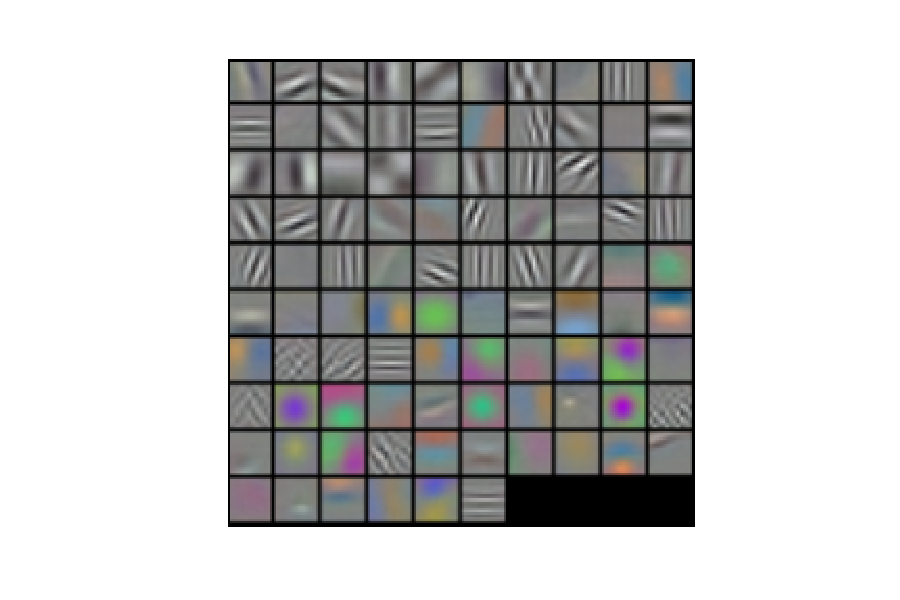
\includegraphics[width=\textwidth]{places205_finetune_layer1.pdf}
	\caption{Layer 1 neurons in fine-tuned PLACES network}
	\label{fig:places}
\end{subfigure}
\begin{subfigure}[t]{0.32\textwidth}
	\centering
	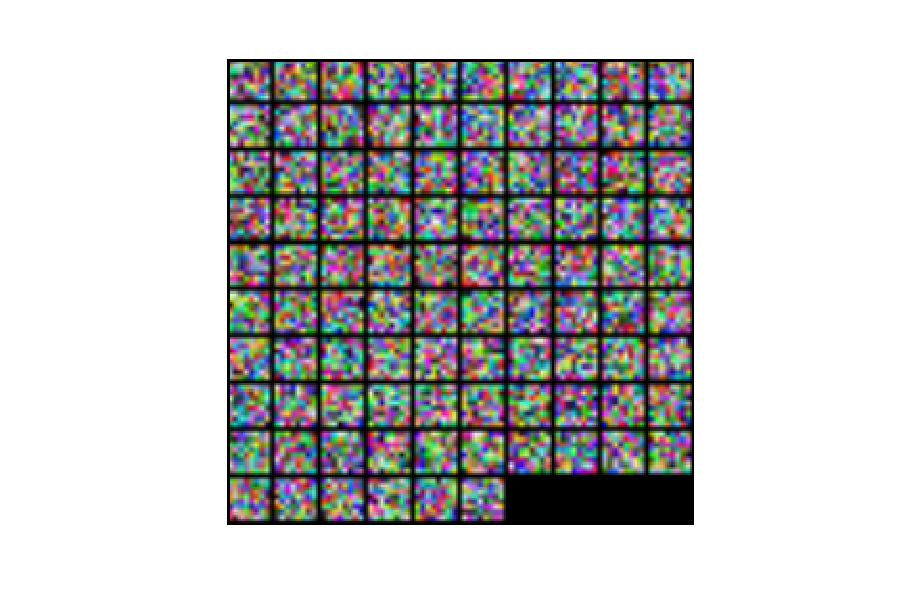
\includegraphics[width=\textwidth]{8_kernel_1_pool_5000_step_iter_50000.pdf}
	\caption{Neurons in single-layer 8 by 8 kernel network without a dropout layer}
	\label{fig:8nodropoff}
\end{subfigure}
\begin{subfigure}[t]{0.32\textwidth}
	\centering
	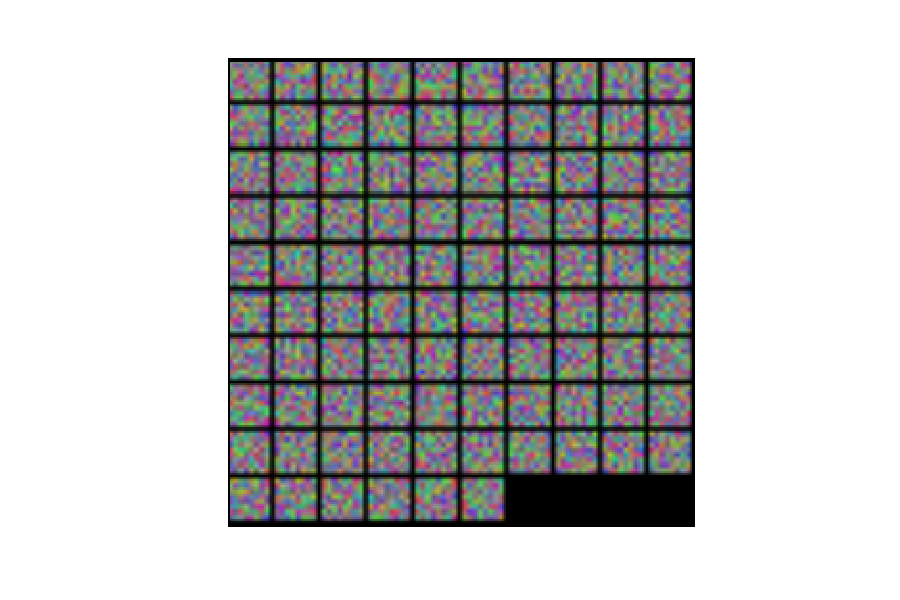
\includegraphics[width=\textwidth]{8_kernel_1_pool_1_dropout_5000_step_5000_after_20000.pdf}
	\caption{Neurons in single-layer 8 by 8 kernel network with a dropout layer}
	\label{fig:8dropoff}
\end{subfigure}
\end{figure}

Even looking at the three-layer network that was trained for 100000 iterations, the neurons in the first layer do not resemble any kind of human-readable structure. In fact, they look similar (and similarly unstructured) to the first-layer neurons in a similar single-layer 12 by 12 kernel network, as seen in Figures \ref{fig:12_6_3} and \ref{fig:12}.

\begin{figure}[!ht]
\centering
\begin{subfigure}[t]{0.3\textwidth}
	\centering
	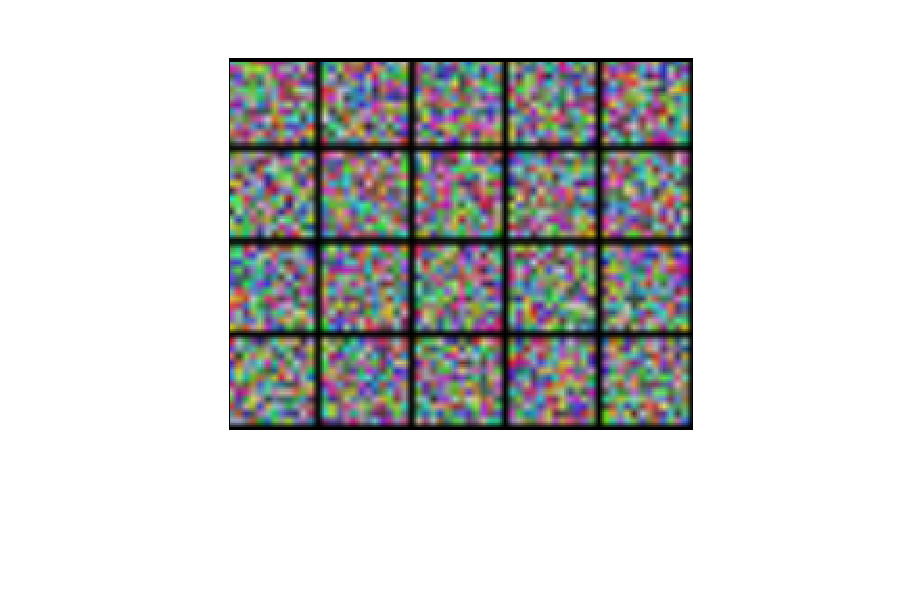
\includegraphics[width=\textwidth]{12_6_3_layer1.pdf}
	\caption{First-layer neurons in a 12x12, then 6x6, then 3x3 kernel network}
	\label{fig:12_6_3}
\end{subfigure}
\hspace{3mm}
\begin{subfigure}[t]{0.288\textwidth}
	\centering
	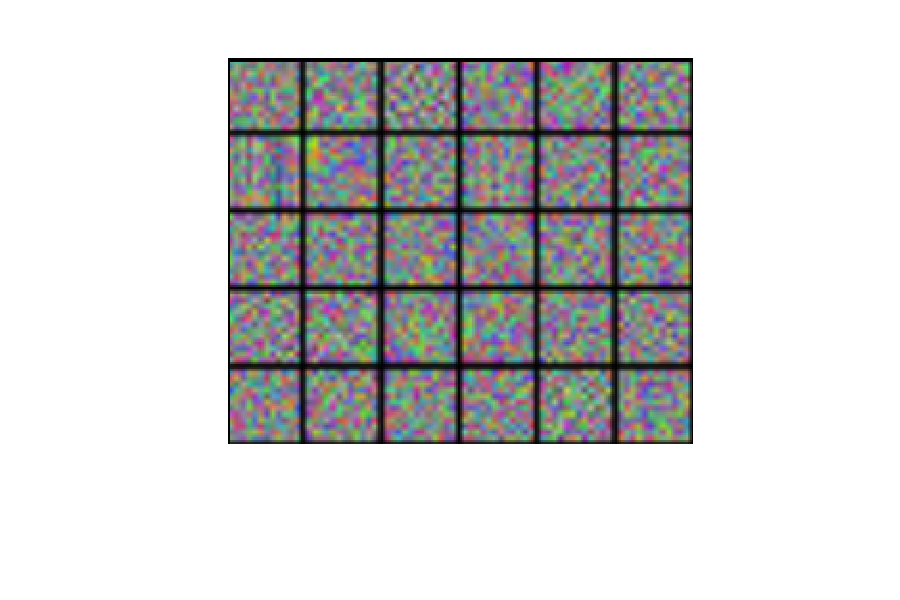
\includegraphics[width=\textwidth]{12_kernel_3_kernel_2_dropout_10000_30_each_1e3_iter_90000.pdf}
	\caption{First-layer neurons in a 12x12 single-layer network}
	\label{fig:12}
\end{subfigure}
\end{figure}

\subsection{Choosing hyperparameters}

To start the hyperparameter optimization process, I started on the 

% * started from hyperparameters given in CNN papers
% * like in 8_kernel_1_pool_1_dropout_10000_step_1e5, optimal learning rate for NNs of comparable size was 0.00001 with dropoff by a factor of 10 every 10000 iterations
% * gaussian processes might have been easier than a grid search
% * use what you know about the domain space - number of classes can dictate the paths of activation that the neurons can take
% * more training and better results in top-5 accuracy. implies that MOAR training will yield better results in top-1 also

\subsection{Mitigating Overfitting}

Additionally, larger networks were less susceptible to overfitting. For example, the 8$\times$8 single-layer kernel network with 96 filters after 50000 iterations had decreased the training set loss to $0.5$, but on the test set showed loss values closer to $6$. Networks with more parameters tend to overfit less, and also using strategies like dropout mitigated this risk. However, the same 8$\times$8 network from above with a dropout layer after the convolutional layer after only 20000 iterations showed a nearly 0 loss on the training set, but reported a loss of over $34$ on the test set. The results were 15 percent top-5 accuracy despite the large test loss, but it is clear that there was an overfitting of the training data. This could have been caused by either a lack of training data, or trying to fit too many parameters in the model.

% TODO: graph of difference between training and test errors to show overfitting? ex: 8_kernel_1_pool_1_dropout_10000_step_1e5.log. and there are others.

\subsection{Overall}

In all, CNNs are very powerful for computer vision tasks, and much more comprehensive work needs to be done in optimizing both shapes of networks and hyperparameter optimization to make neural networks even more powerful than they are today. As technology currently stands, it seems more effective for specific vision tasks to fine-tune a pre-trained network than re-train a simple network to do the same task, since the results are dramatically better.

\bibliographystyle{plain}
\bibliography{6867project}

\end{document}